\begin{figure}[tbp]
\centering
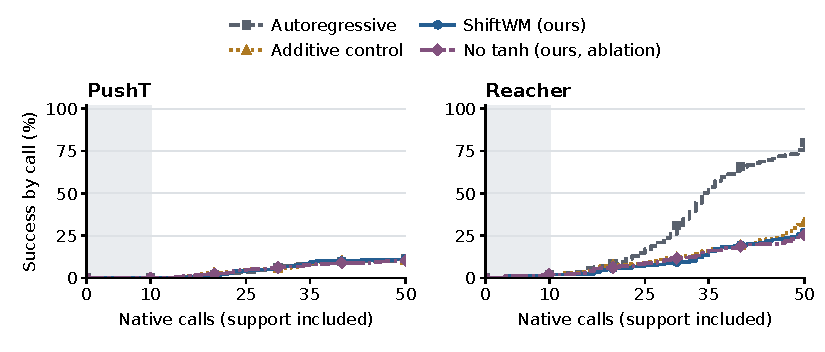
\includegraphics[width=\linewidth]{generated/current_spatial_planning_completion/success_by_budget.pdf}
\caption{Current spatial predictors in closed-loop simulator control. Each curve is the fraction of all 100 test episodes, averaged equally over three training seeds, that has reached the native success criterion by a given call. Failures remain in the denominator. The gray band marks the ten paid support calls; success there precedes policy planning. Every method uses the same goal, start, support controls and CEM $128\times8$/top-16 budget, with 25 then at most 15 policy calls. Curves show point estimates; endpoint uncertainty is in Table~\ref{tab:current-spatial-planning-success}. PushT requires joint pusher/block position error below 20 pixels and circular angle error below $\pi/9$; Reacher requires each unwrapped joint error below 0.05 rad. These are current-spatial results, not the historical context model.}
\label{fig:current-spatial-planning-budget}
\end{figure}
